\documentclass[a4paper, 12pt]{article}
\usepackage[a4paper,top=1.5cm, bottom=1.5cm, left=1cm, right=1cm]{geometry}
\usepackage{cmap}					% поиск в PDF
\usepackage{mathtext} 				% русские буквы в формулах
\usepackage[T2A]{fontenc}			% кодировка
\usepackage[utf8]{inputenc}			% кодировка исходного текста
\usepackage[english,russian]{babel}	% локализация и переносы

\usepackage{amsmath,amssymb}
\usepackage{indentfirst}
\usepackage{longtable}
\usepackage{graphicx}
\usepackage{array}
\usepackage{float}

\usepackage{floatflt}
\usepackage{wrapfig}
\usepackage{siunitx} % Required for alignment
\usepackage{subfigure}
\usepackage{multirow}
\usepackage{rotating}
\usepackage{caption}

\graphicspath{{.}}


\title{\begin{center}Лабораторная работа №3.4.2\end{center}
Закон Кюри-Вейсса}
\author{Рожков А. В.}
\date{\today}

\begin{document}
    \pagenumbering{gobble}
    \maketitle
    \newpage
    \pagenumbering{arabic}

    \textbf{Цель работы:} изучение температурной зависимости магнитной восприимчивости ферромагнетика выше точки Кюри.

    \textbf{В работе используются:} катушка самоиндукции с образцом из гадолиния, термостат, частотомер, цифровой вольтметр, $ LC $-автогенератор, термопара медь-константин.

    \section{Теоретическая часть}
    \paragraph{Модель среднего поля.}
    В качестве простейшей эмпирические модели, описывающей магнитную восприимчивость
    ферромагнетика, можно рассмотреть следующую модель: Пусть намагниченность среды
    пропорциональна некоторому эффективному полю $H_{эфф}$, складывающемуся из поля
    $H$ в данной точке, созданного сторонними токами, и среднего "коллективного"
    поля, пропорционального величине намагниченности $M$
    \begin{equation*}
        M = \chi_{пар} H_{эфф} \\
    \end{equation*}
    \begin{equation*}
        \chi_{пар} \propto 1/T \\
    \end{equation*}
    \begin{equation*}
        H_{эфф} = H + \beta M
    \end{equation*}
    Отсюда можно получить закон Кюри-Вейсса
    \begin{equation}
        \label{Curie-Weiss}
        \chi = \frac{1}{\chi^{-1}_{пар} - \beta} \propto \frac{1}{T - \Theta}
    \end{equation}

    \section{Установка}

    \begin{figure}[h]
        \center{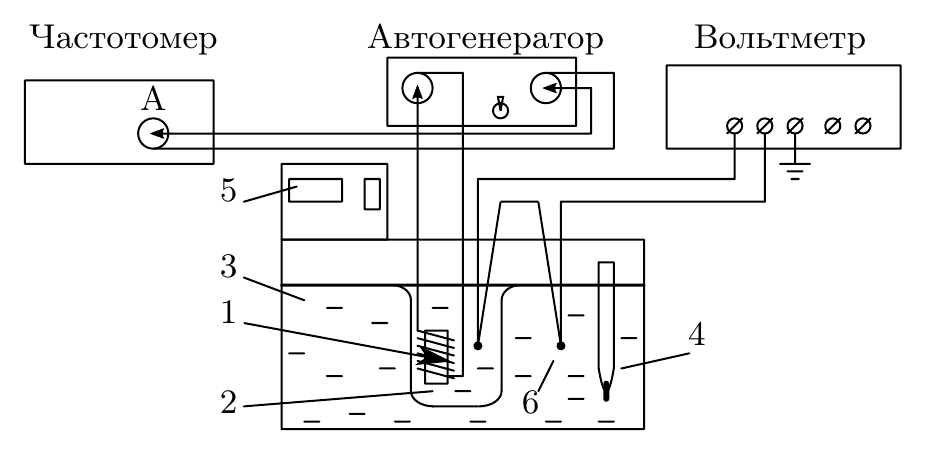
\includegraphics[scale=0.4]{img/ustanovka.png}}
        \caption{Установка для определения коэффициента вязкости жидкости.}
        \label{img:ustanovka}
        \newpage
    \end{figure}


    Установка измеряет температуру образца и собственный период колебания $LC$ контура,
    где $C$ находится в автогенераторе, а в качестве $L$ выступает катушка с гадолиниевым
    сердечником. Обозначим $L_0$ индуктивность катушки без сердечника. Тогда
    \begin{equation*}
        L - L_0 \propto \mu - 1 = \chi
    \end{equation*}
    Так же мы знаем что
    \begin{align*}
        \tau_0 &= 2\pi\sqrt{L_0C} \\
        \tau &= 2\pi\sqrt{LC} \\
    \end{align*}
    Подставляя уравнения и воспользовавшись законом Кюри-Вейсса (\ref{Curie-Weiss}) получаем
    \begin{equation}
        \frac{1}{\chi} \propto \frac{1}{\tau^2 - \tau_0^2} \propto T - \Theta_p
    \end{equation}
    Измерения температуры проводим двумя частями. Термометр измеряет температуру воды в
    термостате, а термопара измеряет разницу температур воды и масла в пробирке, в котором находится образец с катушкой.


\end{document}
